\documentclass[journal]{./template/IEEEtran}
\IEEEoverridecommandlockouts
\usepackage{cite}
\usepackage{amsmath,amssymb,amsfonts}
\usepackage[caption=false]{subfig}
%\usepackage{subcaption}
\usepackage{algorithm}
\usepackage{algorithmic}
\usepackage{graphicx}
\usepackage{textcomp}
\usepackage{xcolor}
\usepackage{url}
\usepackage{comment}
\usepackage{multirow}
\usepackage{commath}
\usepackage[utf8]{inputenc}
\usepackage{kotex}
\def\BibTeX{{\rm B\kern-.05em{\sc i\kern-.025em b}\kern-.08em
    T\kern-.1667em\lower.7ex\hbox{E}\kern-.125emX}}
\begin{document}

\makeatletter

\newcommand\blfootnote[1]{%
  \begingroup
  \renewcommand\thefootnote{}\footnote{#1}%
  \addtocounter{footnote}{-1}%
  \endgroup
}

\newcommand\fs@norules{\def\@fs@cfont{\bfseries}\let\@fs@capt\floatc@ruled
  \def\@fs@pre{}%
  \def\@fs@post{}%
  \def\@fs@mid{\kern3pt}%
  \let\@fs@iftopcapt\iftrue}
\makeatother
\floatstyle{norules}
\restylefloat{algorithm}

\title{Modeling Rotary Unmanned Aerial Vehicle Power Consumption Toward Least-Energy Flight Planning\\
}
\author{
Dooyoung Hong,~\IEEEmembership{Student Member,~IEEE,}
Seonhoon Lee,~\IEEEmembership{Student Member,~IEEE,}
Jaemin Kim*,~\IEEEmembership{Member,~IEEE,}
Naehyuck Chang*,~\IEEEmembership{Fellow,~IEEE,}
\thanks{Direct questions and comments about this article to Jaemin Kim, Myongji University, 116 Myongji-ro, Cheoin-gu, Yongin, Korea (e-mail: jaemin@esl.mju.ac.kr) and Naehyuck Chang, Korea Advanced Institute of Science and Technology, 291, Daehak-ro, Yuseong-gu, Daejeon, Korea (e-mail: naehyuck@cad4x.kaist.ac.kr).}

}
\maketitle
\blfootnote{* Corresponding Authors}

\begin{abstract}
Rotary Unmanned Aerial Vehicles (UAVs), also known as drones, have advantages in various aspects, yet the actual applications are limited due to the flight range. However, it is challenging to increase the flight range through enhancement of the hardware. 
In this paper, we introduce the first step of systematic drone low-power run-time optimization in the framework of electronic design automation (EDA). 
We attempt the drone power management without in-depth knowledge of aerodynamics and control theory. 
Instead, we introduce a novel power modeling of drones using parameters that can affect power consumption such as three-axis velocity and acceleration, the height of drones, wind velocity, the weight and volume of the load. 
This paper presents a detailed experimental setup, power modeling, accuracy verification, and optimization for energy minimum path. 
We achieved over 90\% accuracy in power modeling without depending on the aerodynamics. 
The proposed approach shows the feasibility of energy-aware rotary UAV flight trajectory optimization, and considering the external forces that affect drones such as wind. The proposed method presents up to 12.7~\% energy saving.
\label{Section: abstract}
\end{abstract}














\section{Introduction}
\label{Section: introduction}
The unmanned aerial vehicles (UAVs) are equipped with fixed-wings or rotor wings. 
The fixed-wing methods gain the lift generated by the pressure difference between the upper and lower sides of the wings when the aircraft moves forward. 
The rotor wing method exploits the thrust produced by multiple motors and propellers. Generally, UAVs using the rotor wing method are called drones. 
Unlike the fixed-wing UAVs, drones can take off and land without the restriction of space. 
Modern drones have a built-in flight assistance controller, so even novices can easily control the drones. 
In this paper, we focus on the rotor wing UAVs: drones. We do not mention a long list of drone's advantages in this paper, which is widely known. 

Drones can be equipped with internal combustion engines or batteries as the propulsion power source. In this paper, we narrow down the focus to the battery-operated drones.
Battery-powered drones have various distinct advantages such as zero emission, low noise, and ease of controllability.
Despite those advantages, one of the biggest challenges and limitations of the battery-operated drones is the flight range and time. 
The flight range and time limitation come primarily from the battery energy density, i.e., the energy capacity per unit weight.
In other words, it is hard to scale the flight range and time by simply installing higher capacity batteries as the battery weight also increases linearly by the capacity. 
The weight of the battery is one of the most critical factors for the power consumption of drones. 
Many previous studies have addressed insufficient flight time of drones. 
These efforts aim to increase the flight time through the development of hardware such as motors and batteries~\cite{ref_1}.
Such a component-based approach has led the evolution of drones, but such practices are being matured exhibiting above 90\% efficiency~\cite{ref_2}, which eventually will lose the driving force of drone evolution. 

In this paper, we introduce a system-level approach to enhance flight range and time of drones.
Such an approach is not fundamentally new, but to our knowledge, we are the first to attempt a systematic framework \textbf{inspired by} electronic design automation (EDA) technique.
Unlike previous work, we have elaborated the power consumption model of drones, characterized the power model with the actual flight data of the drone and the effect of external elements such as wind and the load weight, and constructed an accurate simulator.
Such an effort becomes a basis of systematic optimization of drones.
The proposed power model can be easily plugged in linear programming, dynamic programming, and Reinforcement learning (RL) that have been intensely studied to optimize complex design problems with the approximation within a given time complexity.

We figure out the power consumption characteristics of a top-of-the-line commercial drone through dozens of hours of power measurement both on air and on the ground.
We develop a high precision on-board drone power measurement system not to negotiate the measurement fidelity by not using the built-in power measurement feature. 
The power consumption of the drone has been accurately measured using the power measurement board, and a navigation and positioning assistance system called real time kinetic global navigation satellite system (RTK GNSS), which supports the drones global positioning system (GPS), is installed to collect precise flight status data of drones.
We also equip a wind sensor capable of measuring 360 degrees of wind velocity to measure the additional power consumption of drones caused by wind effects during the flight.
We try various ways of data analysis and modeling, and finally, develop a power model using deep learning.
All the modeling process is based on the real flight data of the drone. We develop the power consumption model that has less than 10~\% error, which has been verified with a high precision data acquisition device.

This paper primarily focuses on power measurement, modeling, and characterization, but we also demonstrate optimization method of drones to find the energy-efficient flight paths in a given mission, and we verify the derived energy-efficient paths through the actual flight experiments.
We present an example of saving the energy consumption of the drone by deriving the energy optimal route from the starting point to the destination including the avoidance of an obstacle and proving this by actual flights.














\section{Related works}
% 수식적 방법으로 드론의 최적화를 해결하고자 하는 연구들은 파워 모델과 함께 컨트롤 변수를 이용 하여 시간 진행에 따라 유추되는 파워를 최적화 하는 방식으로 진행하였다. 
% 수식적인 방식은 드론의 연속적인 움직임을 표현하는데 뛰어나지만 현실적인 외란 요소를 가정으로 표현하는 경우가 많고 드론이 운용되는 전체의 시간을 드론이 움직이는 필드까지 가정하여 계산하는데에 많은 시간이 소요된다.
% 그래프 탐색 이론을 이용하여 해결하고자 하는 연구는 드론이 구현된 그래프 내에서 설정 된 각 스탭에 따라 움직이는 과정에서 소비되는 파워가 최소화 되는 루트를 찾는 방식으로 최적화를 진행한다.
% 반면 그래프 서치를 이용한 방식은 드론이 실질적으로 움직일 수 있는 필드와 제약 조건을 구현하기 쉽고 드론의 장시간 운용에 대한 계산을 비교적 쉽게 진행할 수 있지만 구현한 그래프의 각 스텝에 대한 움직임 만을 표현할 수 있기 때문에 스탭 사이의 순간적인 움직임을 유추해내기 힘들며 수식적인 방법에 비해 고 차원의 계산이 매우 힘들기 때문에 파워 모델에 사용 되는 드론의 속도를 고정 하거나 가속도를 배제하는 등의 제한 사항에 의해 수식적 방법에 의해 최적화의 정확도가 떨어진다는 단점이 있다.
%%기존의 방법보다 실용적인 드론의 파워 소비를 최적화 하기 위해서는 드론이 실질적으로 주행 하여야 하는 필드를 시각적으로 표현하기 위한 그래프 서치 알고리즘의 장점과 함께 드론의 움직임을 표현하는 물리적 변수를 최소한으로 사용함에도 직관적이고 보다 높은 정확도를 보이는 모델을 구성하여야 한다.

Previously, drone power management focuses on finding the optimal route between the destinations when a mission of drone is given.
Such practices require to develop the power or energy consumption model first. 
Related literature develops either a theoretical model or a data-driven model from flight experiment data; for example, some researchers focus on aerodynamic characteristics of drones.
They analyze the power consumption due to the propeller drag and the movement of the drone based on fluid mechanics and dynamics~\cite{ref_3}. 
Others who also construct theoretical power consumption models use the traditional power consumption model for hovering rotor-crafts~\cite{ref_4} 
or the relationship between the thrust and revolutions per minute (RPM) of the propeller~\cite{ref_5}. 
It is straightforward to relate the power consumption of drones with the motor torque, current, RPM, and supplied voltage~\cite{ref_6,ref_7}. 
As a white- to gray-box power modeling, the characterization starts from known actual data of drones. For example, C. D. Franco analyzes that the relationship of the power consumption and the velocity of the drone based on a experimental flight data~\cite{ref_8}.  
However, The model assumes that the power consumption for ascending, descending and hovering is constant. Thus, the model is lack of accuracy.
In~\cite{ref_9}, a linear regression model is used to estimate the power consumption for a quad-rotor using on-board power measurement functions. 
However, this causes significant misleading in power modeling according to our measurement.
We mention in Section~\ref{Section: Challenges in drone power measurement} that the data from the factory on-board power measurement of commercial drones is not accurate enough; the resultant power models can potentially impractical and cause false predictions.
We also identify a problem with the data provided by the factory on-board power measurement functions in Section~\ref{Section: Power consumption model for drones}.
Based on the power or energy consumption model of drones, many studies tries to broaden the operation area of drones by minimizing the energy consumption of drones.
In other words, the studies utilize optimization algorithms to minimize the energy consumption of drones and to optimize flight paths to achieve a given purpose or to minimize flight time.
In order to solve the optimization of drones by the numerical method, the studies optimize the total energy over time by using the control variables along with the power model. 
N. Bezzo et al propose Energy-aware planning~\cite{ref_5}. The Model Predictive Controller is used to determine the desired control inputs of the non-linear power consumption model of Helicopter theory that fan thrust is proportional to the square of RPM.
The optimal energy control system derives the minimum energy path through the mathematical solution using the Sequential quadratic programming (SQP) algorithm~\cite{ref_6}. 
In \cite{ref_6}, the model of the control system uses the voltage and torque of the drone motor and the dynamic equations of the drone. 
On the other hand, F. Yacef et al derive the optimal path using the Legendre-Gauss-Radau (LGR) orthogonal collocation method that the numerical algorithm using the motor torque and RPM as major factors affecting the power efficiency and battery life~\cite{ref_7}. 
The optimization of the drone using the numerical algorithm is good for expressing continuous movements, but it cannot reveal unexpected environment variables, which should be measured directly.
On the other hand, the studies to solve the optimization of drones using the graph search theory are optimized by finding a path of drone that minimizes the power consumption as the drone moves according to each step set in the graph. 
Z. Lui focuses on deriving the optimal path using the fast marching method, a variant of the Dijkstra algorithm, and a flight endurance model based on hovering power consumption and battery model~\cite{ref_10}.

Unlike the previous papers, \cite{ref_8,ref_9} established and optimized power consumption model based on the actual flight data of the drone.
Authors measured the power consumption and the speed of drones through experiments \cite{ref_8}. They also expressed the power consumption as a function of speed to derive an energy-efficient aerial flight path using Back-and-forth algorithm.
In \cite{ref_9}, the power consumption is established as a multivariate regression model based on the data measured through actual flight experiments of the drone.
The minimum time path is also derived by considering the battery recharging in the case of multiple destinations.

We present Table~\ref{Table: survay_result} that shows the factors considered for optimization in each study, the algorithms used for the optimization, and the goals of the optimization.
Each study attempted to consider factors that could influence the power consumption of drones externally during the optimization process. 
\begin{table*}[ht]
\caption{Comparison of Previous Works for Drone Optimization.}
\label{Table: survay_result}
\centering
\begin{tabular}{|c|c|c|c|c|c|}
\hline
Reference Paper & Wind & Payload & Surface area & Optimize method & Goal \\ \hline
TVLSI 2019 & O & O & O & Dijkstra algorithm & \multicolumn{1}{l|}{minimum energy} \\ \hline
ICARSC 2015 {[}7{]} & - & - & - & Back-and-forth algorithm & minimum energy \\ \hline
IROS 2016 {[}5{]} & O  & - & - & Model predictive control & minimum energy \\ \hline
ICRA 2016 {[}6{]} & - & O & - & SQP algorithm & minimum energy \\ \hline
IMAV 2017 {[}8{]} & - & O & O & LGR orthogonal collocation & optimal path \\ \hline
SysCon 2017 {[}10{]} & O & - & - & fast marching method & optimal path \\ \hline
arXiv 2017 {[}9{]} & O & O & - & Dynamic graph algorithm & minimum time \\ \hline
\end{tabular}
\end{table*}

We use graph search method to optimize the drone movement. The graph search method is easy to implement the fields and constraint on which the drones can move, and can easily calculate the long-term operation of drones in the implemented graph.
However, since the movement of drone is limited to each step of the graph, it is difficult to infer the continuous movement of the drone in the step, and it is also difficult to calculate the high dimension that can’t be visualized so that the speed or direction is fixed to reduce the dimensions.
The heuristic that fixes the speed and direction limits the degree of freedom of drones and adversely affects the results of optimization due to limited movement.
Thus, we should consider the following that: 
\begin{itemize}
    \item The power consumption model should be composed of a more intuitive and highly accurate model that uses a minimum of physical variables of the drone than a numerical method using a complicated formula to express the movement of the drone.
    \item The proposed optimization method has to use the advantage of the graph search algorithm that can take into account environment variables from the real data and is easy to calculate for long-term operation of drones.
    \item Heuristics should be applied to reduce the optimal path calculation cost or to find an approximate solution when classic methods fail to find any exact solution.
\end{itemize}

In this study, unlike previous studies such as~\cite{ref_9}, we collect the drone's power consumption data based on the accurate power measurement board manufactured by ourselves. 
Additionally, we install RTK GNSS to assist the basic GPS on the drone to collect the accurate flight status data. We also install the wind sensor on the drone to directly measure wind, which affects the power consumption of the drone.
We include the weight of the load on the drone and surface area increased by the load as a factor in the power consumption model of the drone.
We set power consumption model input variables as three-axis velocity, acceleration over time, total drone weight, the volume of a delivery load, and wind velocity collected by the wind sensor.
We predict the exact power consumption of drone without knowledge of complex aerodynamics or complicated calculations by using a neural network that is trained by real flight data such as drone velocity, acceleration, and so on.
After that, we implement the power consumption model that infers the accurate power consumption of drone during the flight using deep neural networks and confirm the accuracy of the power consumption model through actual flight.
Finally, based on the established model, we present an example of a complex drone energy optimization using the Dijkstra algorithm to derive an energy-optimized route to the destination in given scenarios with various obstacles imparted by wind fields.

\label{Section: Related works}














\section{Challenges in drone power measurement}
\label{Section: Challenges in drone power measurement}

\subsection{Inaccurate data from genuine flight computer}
Top-of-the-line commercial drones provide flight data such as power consumption and GPS location during the flight. 
We use the DJI Matrice 600 Pro (M600), which is a flagship model of DJI~\cite{ref_11}, one of the world-leading drone companies. 
M600 is equipped with A3 flight control module that includes an on-board data logger for the flight data at a sampling rate of 200 Hz. However, it turns out that the factory data logger is not accurate enough to build a power model. It goes without saying that the flight data should be accurate to build a useful power consumption model.
Therefore, we check the data from the A3 module securing the drone on the ground without turning on the propulsion using a high precision data acquisition device (NI DAQ)~\cite{ref_12}.

\begin{table}[ht]
\caption{An example of inaccurate data from the genuine flight module of M600 drone while it parks as a ready state on the ground. (All motors and propellers are fully stopped.)}
\label{Table: motor_status}
\resizebox{0.485\textwidth}{!}{%
\begin{tabular}{|c|c|c|c|c|c|c|}
\hline
Motor number & Motor 1 & Motor 2 & Motor 3 & Motor 4 & Motor 5 & Motor 6 \\ \hline
Voltage (V)  & 51.3 & 51.1 & 51 & 51.5 & 51.4 & 51.1 \\ \hline
Current (A)  & -0.05 & -0.57 & -0.15 & 0.19 & 0 & 0.45 \\ \hline
Power (W)    & -2.56 & -29.12 & -7.65 & 9.78 & 0 & 22.99 \\ \hline
\end{tabular}%
}
\end{table}

The measured value in Table~\ref{Table: motor_status} shows non-negligible negative current values, which indicates the battery of the drone is being charged.
It is impossible to charge or discharge a drone without any movement, this explains that there is a distinct DC offset in the power measurement circuit.
To check the DC offset correctly, we measure the power consumption of the drone during propulsion by tightly securing the drone on the ground while increasing the throttle.

\begin{figure}[ht]
\centering
\subfloat[The power measurement test on the ground.]{\includegraphics[scale=0.9]{fig1/Ground_test.pdf}}
\qquad
\subfloat[Comparison of the current flow between NI DAQ and on board measurement.]{\includegraphics[scale=1.0]{fig1/NIvsDJI.pdf}}
\caption{Experiment set for the power measurement on the ground and the result.}
\label{fig:Ground_test}
\end{figure}

Fig.~\ref{fig:Ground_test}(a) shows the shunt resistor and the operational amplifier (OP-AMP) for the current measurement. 
The experiment result is presented in Fig.~\ref{fig:Ground_test}(b). 
It visualizes that the current profile of the factory on board power measurement circuit is marginally similar to that of the high precision data acquisition device, but the actual scale is significantly different. 

To overcome this difference, we attempt various trials to use the on board power measurement circuit by post-processing (calibration, etc.). But, the source of error is not only the DC bias and gain error, but also sampling rate and linearity. 
We conclude that the on board power measurement circuit in the drone is not appropriate for the research we aim at because of the inaccurate power data. 
As a result, the power consumption model also becomes inaccurate, and in turn, the derived energy-efficient flight route through the power consumption model incurs wrong results as well.





\subsection{Design the power measurement board}
We design the power measurement board to exhibit a very high accuracy like the high precision data acquisition device. 
We select parts to ensure the accuracy, and we also verify the measured data by comparing it with that of the same high precision data acquisition device, which is used for the evaluation of the DJI on board power measurement circuit.
We configure a power measurement board with a combination of devices and circuits and built a real-time operating system (RTOS) on a micro controller unit (MCU) to schedule the operation of the MCU in a hard time. 
The configured power measurement board is lightweight and separated battery-powered so that doesn't affect the power consumption of the drone.

\begin{figure}[ht]
\centering
\subfloat[The front side of the measurement board.]{\includegraphics[scale=0.20]{fig2/New_board_front.pdf}}
\subfloat[The back side of the measurement board.]{\includegraphics[scale=0.20]{fig2/New_board_back.pdf}}
\caption{The power measurement board installed on the drone.}
\label{fig:board}
\end{figure}

The power measurement board acquires the battery voltage under an upper limit of 52~V, at which the target drone is driven by using the analog to digital converter (ADC) of the MCU. The power measurement board also acquires the current using with a 1~milliohm shunt resistor and an amplifier.
The values of measured voltage and current are stored to the SD card as the binary format file that is easily processed externally.
All measurement tasks on the power measurement board store data at a sampling rate of 1~kHz under the management of FreeRTOS real time operating system.
Fig.~\ref{fig:board} shows components of the completed power measurement board.

\begin{figure}[ht]
\centering
\includegraphics[scale=0.8]{fig3/flight_experiment.pdf}
\caption{The power measurement test during flight.}
\label{fig:flight_test}
\end{figure}

\begin{figure}[ht]
\centering
\includegraphics[scale=1.0]{fig4/flight_exp_result.pdf}
\caption{Comparison of the current measurement by each measurement device. The power measurement board presents data as accurate as NI DAQ.}
\end{figure}
\label{Section: Design the power measurement board}

Fig.~\ref{fig:flight_test} illustrates how we measure the power consumption data of the drone in flight.
The measured current value on the power measurement board has an error of less than 6\% compared with the high precision data acquisition device. By installing a light weight power measurement board with high accuracy on the drone, we collect power data instead of the incorrect on board genuine flight computer.





\subsection{RTK GNSS and wind sensor}
We use the physical parameters such as speed, acceleration, and so on to construct the power consumption model of drones.
The commercial drones leave these parameters in the back log data to record their flight status.
To acquire the parameters, we synchronize the on board genuine flight computer and our light weight power measurement board together. In general, the drone determines the position through the inertial measurement unit (IMU) and GPS modules. 
However, the factory on-board GPS module on M600 has a vertical error of 0.5 m and a horizontal error of 1.5 m, respectively. 
Such an amount of positional errors reduce power model accuracy.
To enhance the accuracy of commercial GPS, real time kinetic (RTK) assistance GNSS is developed. Under the assistance of ground GPS station, RTK GNSS enhances the GPS accuracy to reduce the error to the order of cm. We use DJI's optional RTK GNSS module~\cite{ref_13}.
We install RTK GNSS on the drone and validate the improved accuracy by comparing it with another separate industrial high precision GPS module~\cite{ref_14}.
To measure the error of GPS, we conduct following simple experiment. First, we collocate the antenna of the industrial high precision GPS module and the drone on the same positions. Then we shift both the industrial GPS module and the drone by a specific distance and compare the actual distance with calculated distance values from the industrial GPS module and the drone.
As a result of the experiment, we verify that the RTK GNSS on drone has less than 5 cm error in any case compared with the industrial GPS module. This error is about 20 times lower than the error of the drone on-board GPS.

On the other hand, the wind highly affects the power consumption of drones as well as the other parameters such as velocity, acceleration, and so on.
It is necessary to take account in this effect as a factor in the power consumption model of drones. 
If a drone flies in the same direction as the wind, the drone consumes less power; if the drone flies in the opposite direction, the power consumption increases as the air resistance increases. 
This phenomenon becomes more severe while the overall surface area of drone increases as we mention in Section~\ref{Section: Power consumption model for drones}.

However, measuring wind speed and direction in real-time is very difficult because turbulence frequently occurs at high altitudes in which the drone fly, and the effects of air irregularities on the drone are unpredictable.
So, many studies conduct experiments using artificial wind or wind information of the area where the drone is flying provided by the national meteorological agency~\cite{ref_5,ref_9}. 
Nevertheless, it is true that in the real situation, the drone encounters the turbulence that changes drone's altitude or velocity; so, if the drone does not have a tool to measure the influence of the wind, wind direction and speed cannot be used as a actual factor in the power consumption model of the drone. 

\begin{figure}[ht]
\centering\includegraphics[scale=0.8]{fig5/wind_sensor.pdf}
\caption{The picture of installed wind sensor FT-205 and DJI's RTK GNSS}
\label{fig:wind_sensor}
\end{figure}

In this work, we measure the actual wind, which affects the drone's power consumption. We attach a wind sensor FT205~\cite{ref_15} in Fig.~\ref{fig:wind_sensor} on the drone. 
The wind sensor measures the direction and speed of the wind affecting drones with a sampling rate of 10 Hz and a maximum error of 0.3 m/s.
The wind data measured by wind sensor is also stored in SD card of power measurement board with power consumption data of drones.











\section{Power consumption model for drones}
\label{Section: Power consumption model for drones}
As we mentioned in Section~\ref{Section: Related works}, power consumption models of drones can be classified into the aerodynamics based modeling or the motor power based modeling or the data-based modeling. 
Each modeling method derive the parameters necessary for each method through the specification or data measurement of drones and uses them for model formation.
The power consumption model based on aerodynamics can describe the flight of aircraft as a physical phenomenon, expressing the principle of power consumption as a force in a horizontal direction and a force for rotation, to clearly express the factors affecting power consumption. 
However, coefficients for expressing these force (e.g. air resistance, motor efficiency, and propeller efficiency) can’t be obtained by simple measurements. 
Since the coefficients and specifications of non-measurable drone parameters only depend on the information provided by the manufacturer of the component, the power consumption of the model based on this information may differ from the actual power usage.
In addition, the aerodynamic-based model can’t directly consider disturbance that has a huge impact on the power consumption of drones during the actual flight.
Therefore, there is a difference between the power consumption measured in actual flight and the power consumption predicted by the aerodynamics model.
On the contrary, the model using the theory that infers the power consumption from the thrust of motor and the propeller has very high accuracy because the power consumption and the power source are directly related, but the momentum theory is only valid for the calculation of the thrust with hovering state of drones. 
It is difficult to apply to drones that must fly in multiple direction to perform~\cite{ref_4}.

Although the data-driven modeling method requires a lot of actual measurement data to build the model, the constructed model has high accuracy if the collected amount of data is a lot and it's accurate enough.
A built model using such method can accurately predict the power consumption of a drone without knowledge of aerodynamics or complicated calculations if the variables that can highly affect the power consumption (e.g. velocity, acceleration, disturbance, etc.) are properly selected as the inputs of the model.
We use the deep neural networks, one of the techniques of machine learning, to build a model based on the power consumption data and other measurable parameters that affect the power consumption of drone collected in Section~\ref{Section: Challenges in drone power measurement}.
The deep neural network models a function in the form of a black box. The model is constructed using simple parameters that can represent the motion of the drone instead of the theory-based formulas as in the conventional regression method. 
Besides, since neural networks can theoretically approximate all functions, it is possible to predict the complex power consumption process of drones well.
In this section, we present the grid search process that finds the optimal inputs and structure of the neural network to construct an optimized model. 
We also verify the power consumption model and show the accuracy of the model on the four kinds of benchmark flights.





\subsection{Deep neural network}
The Deep Neural Network (DNN) is the technique that automatically constructs the model as the form of a black box by complex mathematical equations when data is input.
The algorithm can predict and classify a target based on the attributes learned through training data. 
Deep neural networks consist of several hidden layers between the input layer and the output layer.
As the hidden layers become deeper, the characteristics of the input data can be more abstracted through each hidden layer.
The DNNs can extract characteristics from input data and create a complex model with few data elements, unlike the conventional data regression methods.

However, DNNs have a disadvantage in that the complex relationship between the input set and the neural net structure is unknown since it is based on a black-box model. 
Therefore, there is no clear criterion on how to select the hyper-parameters such as learning rate, hidden layers, and the number of neurons to construct the optimal structure of the deep neural network. 
When constructing a model for power consumption prediction using DNNs, the hyper-parameters of neural networks should be set optimally to increase the accuracy of the model and prevent over-fitting between the model and training data to minimize the adverse effects on the model.
To find optimized hyper-parameters of DNNs, users should repeat the sequence searching the hyper-parameters of the neural network. 
The most frequently used methods of optimizing the hyper-parameters of DNNs are the random search method and the grid search method~\cite{ref_16}. 

The grid search method is an exhaustive hyper-parameter search with pre-set range and interval. The method tries every possible combination of hyper-parameters in the given range and interval and records the performance metric for each combination. 
By comparison, the random search method generates a combination of hyper-parameters using random numbers so that the combination of hyper-parameters can be searched much faster than the grid search method that searches all cases of hyper-parameters. However, the random search method has a significant disadvantage that the optimal result of the random search method varies depending on a range of arbitrary hyper-parameters, which is set by the user.

We use the grid search method that obtains the best result in a given space and then we record the performance metric as Root Mean Squared Error Percentage (RMSEP) for each hyper-parameter combination.
The configured input variables of the deep neural networks are three-axis velocity and acceleration, altitude, the total weight of the drone, two-axis wind velocity, and surface area of loads. 
We evaluate various combinations of the model parameters by the cross-validation results and determine the combination with the lowest error. 
The model parameters such as learning rate, the number of hidden layers, and the number of hidden neurons, have no specific rules for networks structure and should differ among applications. 

We search the number of hidden layer from 3 to 70 and the number of hidden neurons from 10 to 100. 
The learning rate is progressed by decaying the learning rate function in the TensorFlow from 0.01 and the batch size is gradually increased by a power of 2 from 64 to 4096.
We use both the Rectified Linear Unit (ReLU) and the linear function as activation functions for the hidden layers and the output layer respectively. 
Also, we use ADAM and SGD algorithm are used as candidate for the learning algorithms~\cite{ref_17}. 
We train the DNNs with 30 hours of data. Randomly excluded 0.5\% of the total data is remained for the validation of the trained model.
The grid search is performed for 370 hours on the system consists of Intel\textregistered ~i7-8086K CPU @ 4.00~GHz (12 cores) and NVIDIA\textregistered ~GeForce 1080Ti 16~GB.

After recording the measured performance for each hyper-parameter set (combination), we select the hyper-parameter set (combination) that performed the highest performance. 
Table~\ref{Table: gridsearch_result} shows a top 7 accuracy ranking list of hyper-parameter sets (combinations) of neural networks.

\begin{table}[ht]
\caption{The list of grid search results}
\label{Table: gridsearch_result}
\resizebox{0.485\textwidth}{!}{%
\begin{tabular}{|c|c|c|c|c|c|l|}
\hline
Epoch & Learning late & Neurons & Hidden layers & batch size & Optimizer & {RMSEP} \\ \hline
690   & 0.0005  & 44 & 35 & 2048 & Adam & 8.37526 \\ \hline
494   & 0.001   & 60 & 60 & 2048 & Adam & 8.40487 \\ \hline
277   & 0.0003  & 80 & 60 & 2048 & Adam & 8.42413 \\ \hline
794   & 0.0002  & 44 & 35 & 4096 & Adam & 8.45175 \\ \hline
709   & 0.001   & 44 & 30 & 512  & Adam & 8.46091 \\ \hline
844   & 0.005   & 36 & 25 & 4096 & Adam & 8.51061 \\ \hline
577   & 0.0005  & 36 & 35 & 512  & Adam & 8.52163 \\ \hline
\end{tabular}%
}
\end{table}

As a result, the accuracy of neural networks using 0.0005 learning rate, 44 neurons, 35 hidden layers, 2048 batch size, ReLU for activation function, and ADAM for learning algorithm was the highest. Fig.~\ref{fig:DNN_structure} shows DNNs structure with optimized hyper-parameters.

\begin{figure}[htbp]
\centering\includegraphics[scale=0.25]{fig6/NN_structure.pdf}
\caption{DNNs structure with optimized hyper-parameters}
\label{fig:DNN_structure}
\end{figure}

\label{Section: Deep Neural networks (DNN)}





\subsection{Validation of power consumption model}

We configure the environment of the drone flight for verifying our power consumption model. 
The on board SDK provided by DJI is used in conjunction with the meta software Robot Operating System (ROS), which is used in the robotics field, to simulate the automatic driving of drones. 
Autonomous driving simulation of the drone through the program is much easier to adjust the velocity and acceleration required for the drone operation than the user can directly control the controller. 
Fig.~\ref{fig:SDK} shows the on board SDK environment of M600 for autonomous driving simulation.

\begin{figure}[htbp]
\centering\includegraphics[scale=0.36]{fig7/SDK.pdf}
\caption{The on board SDK system for automatic flight of drones}
\label{fig:SDK}
\end{figure}

In order to validate the accuracy of the power consumption model, we upload the autonomous driving simulation program to the drone to perform the actual flight and compare the power consumption predicted by the power consumption model with the actual power consumption. 

\begin{figure}[ht]
\centering
\subfloat[Drone power consumption when hovering.]{\centering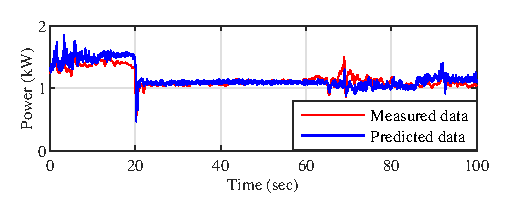
\includegraphics[scale=1.05]{fig8/Hover8x3.eps}}
\qquad
\subfloat[Drone power consumption when ascending and descending.]{\centering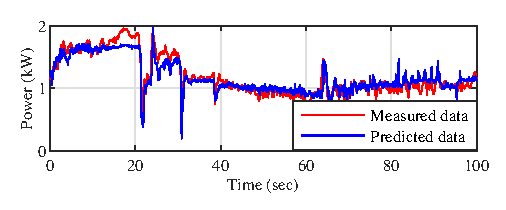
\includegraphics[scale=1.05]{fig8/AD8x3.eps}}
\qquad
\subfloat[Drone power consumption when interval flight.]{\centering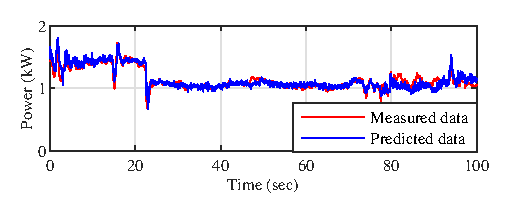
\includegraphics[scale=1.05]{fig8/Interval8x3.eps}}
\qquad
\subfloat[Drone power consumption when squared-shaped flight.]{\centering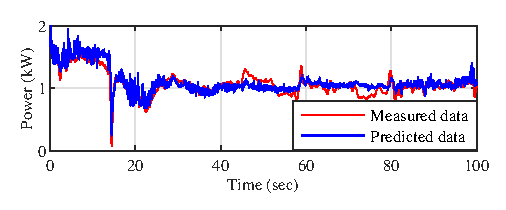
\includegraphics[scale=1.05]{fig8/Square8x3.eps}}
\caption{Comparison of measured power consumption and predicted power consumption under the benchmark flights.}
\label{fig: benchmark}
\end{figure}

Fig.~\ref{fig: benchmark} shows the measured power and estimated power when i) the drone is hovering in the air, ii) the drone repeats vertical flights (ascending and descending without horizontal movement), iii) the drone is flying an interval flight path that repeats horizontal flights (straight flight and back straight flight without vertical movement), and iv) the drone is flying a rectangular and level flight path, respectively. 
We compare the power estimated by the proposed power model with the measured flight data and confirm that the error of each benchmark test is 6.27\%, 9.8\%, 7.82\%, and 9.12\%, respectively.





\subsection{Effect of weight and surface area on drones}
% 우리는 수집 된 데이터를 기반으로 taget drone 인 M600이 translational lift의 효과를 받아 에너지를 효율적으로 활용 할 수 있는 드론의 속도 구간을 제시 한다. 베이스 라인은 드론에 어떠한 부착물 없이 등속을 유지하는 상태에서 바람 센서가 바람의 영향이 없을 정도 (0 ~ 1 m/s)의 세기를 기록할 때 드론의 등속도 대비 거리 당 소비한 에너지이다.
% 무게 라인은 드론에 부하가 걸린 상태에서 등속을 유지히며 드론에 어떠한 부착물 없이 등속을 유지하는 상태에서 바람 센서가 바람의 영향이 없을 정도 (0 ~ 1 m/s)의 세기를 기록할 때 등속도 대비 거리 당 소비한 에너지이다.
% 윈드 라인은 두 라인과는 다르게, 바람 센서가 드론의 방향의 반대쪽의 6 m/s의 세기를 기록할 때 드론의 등속도 대비 거리 당 소비한 에너지이다.
%이 후 Fig. 10 처럼 드론에 외부 영향을 가했을 때 속도 구간이 변하는 모습을 기록한다.
It is very important to consider the weight of the aircraft and the effects of wind, when referring to aircraft such as drones.
As the total weight of a drone increases, the thrust demanded by the drone to perform the flight increases, increasing the power consumption of the drone. 
Also, when a drone delivers a payload, the wind resistance increases by the surface area of the shipment, which also affects power consumption.
We collect data by varying the shape of boxes and the weight of payloads and then include the collected data in the training data of the power consumption model.
Also, too heavy loads are very inefficient to be transported by drone, so the experiment was carried out by adding up to 2kg, which is about half the weight that M600 can carry.

\begin{figure}[ht]
\centering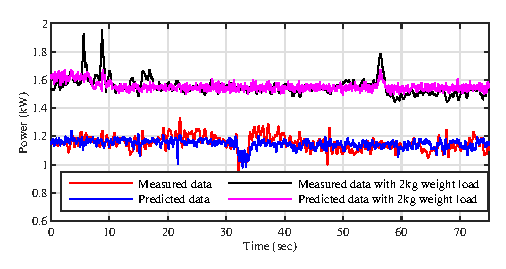
\includegraphics[scale=1.1]{fig9/compare_weight8x4.eps}
\caption{Comparison result of the power consumption model with payload and without payload during constant velocity flight of 6 m/s.}
\label{fig: Model_weight}
\end{figure}

Fig.~\ref{fig: Model_weight} shows the result of estimating the power consumed by a drone with the payload during constant velocity flight and the power consumed by a drone without payload in the same flight condition. The model has less than 10~\% error in each case. 
When comparing the results, the drone consumes about 30~\% more power, despite adding only 2 kg, half the maximum loadable weight of M600, which means the run-time of the drone is also reduced by the same rate.

To confirm the changes in the power consumption of the drones due to the increase in the surface area, we identify the optimum energy velocity of the drones inferred by the Helicopter effective translational lift.
Helicopter effective translational lift, commonly called translational lift in aerodynamics, always occurs when the rotor blades move horizontally. When an aircraft with a rotor-craft moves at a certain velocity, no vortices occur in the rotor-craft and the air flows horizontally, and the lift force increases due to the airflow, and the induced drag of the aircraft decreases. 
This additional lift at a certain velocity is called effective translational lift, and this characteristic is affected by the aircraft's characteristics (weight, surface area, etc.). 
The translational lift should be used when operating the aircraft at maximum performance~\cite{ref_20}.
Based on the collected data, we present the velocity range in which the M600 can efficiently utilize energy under the effect of translational lift. 
The baseline is the energy consumed per distance versus the constant velocity of the drone without any payload when the wind sensor records the weak wind speed between 0~m/s to 1~m/s that the wind does not affect the power consumption of drone.
The weight line is the energy consumed per distance versus the constant velocity of the drone with the payload of 2~kg when the wind sensor records the weak wind speed between 0~m/s to 1~m/s.
Unlike the two lines, the wind line is the energy consumed per distance versus the constant velocity of the drone without the payload when the wind sensor records the strong wind speed between 6~m/s to 8~m/s. 
As shown Fig.~\ref{fig: lift}, we propose how the speed range changes when an external influence is applied to the drone.

\begin{figure}[ht]
\centering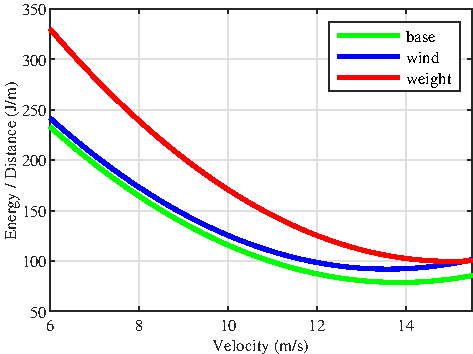
\includegraphics[scale=1.0]{fig10/t_lift.eps}
\caption{The effect of The translational lift on the optimal velocity for the least energy consumption per a meter.}
\label{fig: lift}
\end{figure}

Initially, the drone has an optimum velocity that consumes the least energy without external external attachments. 
When the box is added, the overall surface area of the drone increases, the drag force received by the drone increases, increasing the overall power consumption and also decreasing the optimal speed slightly. 
Adding weight to the drone greatly increase the overall power consumption of the drone and increase its optimal velocity.
As the above results, the drone has various optimum flight velocity according to the environment, and the optimal method of operating the drone can be determined by combining the optimum flight velocity and the battery consumption of the drone. 
Therefore, it is very important that the power consumption model correctly represents the fluctuations in power consumption due to the weight and wind. 
The power consumption model that can infer power consumption in any environment is the basis for optimizing the energy consumption of the drone.

% 그러나 드론에 무게를 추가한 경우에는 translational lift effect에 기반한 거리 대비 에너지 최적 속도가 M600의 안전 운용 범위 (바람이 없는 상태에서 최대 18 m/s) 밖으로 벗어난다. 때문에 실험을 진행하지 않고 차후 이종 드론을 취급 할 때 소형 드론을 이용한 실험을 통해 진행 할 것이다. 무게에 의한 영향에 인한 전력 소비 비교와 경로의 변화 탐색은 우리의 다음 일로 남겨둔다.

Note that when weight is added to the drone, the velocity based on the translational lift becomes outside on the M600's safe operating range (up to 18 m/s without the wind). Unavoidably, we cannot experiment in this paper to determine the effect of payload weight because of a safety issue. But later, we will proceed with experiments using small drones to handle heterogeneous drones.










\section{Flight energy optimization and its validation}

We predict the energy consumption when a drone arrives from a starting point to a designated destination, avoiding obstacles encountered while flying downtown from an energy efficiency point of view. After deriving a flight path that consumes the least energy based on the power consumption model, we validate the usefulness of the our optimization method of drone by flying the derived path to a real drone and comparing the energy consumption.
As we mentioned in Section~\ref{Section: Related works}, there are advantages and disadvantages to the method of optimizing drones through numerical algorithm and the method of optimizing drones through graph algorithms.
However, to optimize the overall operation of the drones, the optimization method must be able to consider both the environment and the time of drone operation. 
The numerical algorithm is good for expressing the momentary movements of the drone, but it is not suitable for calculating all the movements of the drone about half an hour at wide range.
Therefore, we optimize the overall movement of the drone by using a graph algorithm that can visualize the external environment of the drone.





\subsection{Configuration of optimization problem}

%% 이미 챕터 2에서 언급하였듯이 수식적으로 드론의 최적화를 진행하는 방법과 그래프 알고리즘을 통하여 드론의 최적화를 진행하는 각 방법에는 장, 단점이 존재한다.하지만 드론의 전체적인 운용과정 최적화하기 위해서는 드론이 움직이는 환경과 시간을 둘 다 고려할 수 있어야 한다. 수식적 방법은 드론의 순간적인 움직임을 표현하는데 뛰어나지만 넓은 범위에서 약 반 시간에 해당되는 드론의 모든 움직임을 계산하기엔 적합하지 않기 때문에 드론의 외부 환경을 시각화 시킬 수 있는 그래프 알고리즘을 이용하는 편이 최적화에 용이하다.
%%우리는 드론이 실제 주행하는 환경을 고려하여 (지구 곡률 반경의 영향은 없다는 가정 하에) 노드와 모서리로 구성된 3차원 탐색 공간의 그래프로 구성하였다.
% 그림 a는 노드와 엣지로 구성 된 그래프의 일부이다. 노드는 드론의 파라미터와 외부 환경 요소를 포함하며 포함한 모든 요소들의 경우의 수만큼 엣지를 지닌다. 엣지는 노드 사이를 움직 일 수 있는 경로이며, 엣지에 부여된 가중치들을 비교하며 드론의 진행 경로를 결정할 수 있다.  그림 b는 노드와 엣지로 구성 된 그래프를 기반으로 드론이 움직이는 환경을 구성한 것이다.

%% 그래프는 X축과 Y축의 범위가 250m 이고 Z축이 100m 인 공간에 시작점과 끝점 사이에 여러 형태의 건물이 있다는 것을 가정하여 드론이 접근 할 수 없는 구역을 설정하였다. 드론은 그래프의 각 스탭에 따라 평면으로 이동할 경우 각 축의 1스텝마다 10m씩 이동하며 수직 이동 할 경우 수직 축의 1스텝마다 3m씩 이동이 가능하다.
%%그래프 내에서 드론이 현재 스탭에서 다음의 스탭으로 진행할 수 있는 방향은 그림 12와 같이 총 26가지 이지만 드론의 최적 경로를 탐색하는 경우, 드론이 운용시간이 길어 질수록 에너지를 더욱 많이 소비하기 때문에 드론의 주행 경로를 연장시키는 후진에 대한 경우의 수를 모두 배제하여야 한다. 따라서 드론이 다음 스탭으로 나아갈 수 있는 방향은 총 17가지 이다.
%% 노드 사이를 이동하는 드론의 속도는 fig 10의 helicopter translational lift 현상을 기반으로 M600이 거리 당 에너지를 최소로 소모하는 속도를 기준으로 탐색한다. M600이 에너지를 최소로 소모하는 속도는 외부 영향에 의하여 언제든지 변할 수 있으며 이를 고려하기 위해 속도의 탐색 범위를 최소 6 m/s 부터 최대 15 m/s 까지 설정하였다.
%% 그래프 서치 알고리즘을 사용하는 연구들은 스탭 사이를 이동하는 물체의 순간적인 움직임을 계산하기 어렵기 때문에 물체가 노드 사이를 등속도로 움직인다고 가정한다. 하지만 드론은 모터의 출력이 높아져 기체가 수직 혹은 수평으로가속하는 순간이 가장 파워를 많이 소비 하기 때문에 우리는 드론의 가속도가 파워 소비에 미치는 영향을 고려 할 수 있게끔 제작한 파워 소비 모델을 기반한 최적화 문제를 구성한다. 최적화 문제의 풀이 과정 중 가속도를 고려하기 위할 때 생기는 문제점과 해결을 위해 적용한 휴리스틱은 섹션 B에서 언급한다.
% 구성하는 드론 최적화 문제는 드론이 스타팅 포인트에서 비행을 시작하여 그래프의 각 스탭에서 에너지를 최소로 소모하는 경로를 탐색하면서 end point에 도달 하는것이 목표이며, 바람의 세기같은 외력이 드론에 작용 할 때에도 드론이 외력에 대응하여 에너지를 덜 소모하는 최적의 경로를 도출 하는 것이다.
%% 최적화 알고리즘은 다익스트라 알고리즘을 사용한다. 다익스트라 알고리즘은 exhaustive search를 이용한다. 

\begin{figure}[ht]
\centering
\subfloat[The isometric view of the visualization of the environment around which drones fly.]{\centering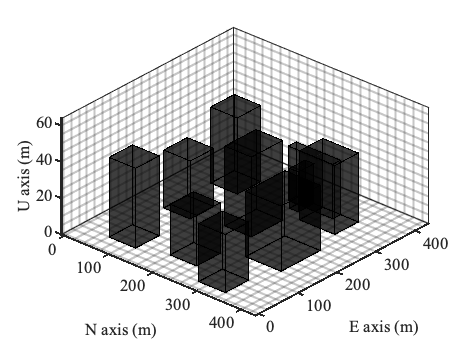
\includegraphics[scale=1.0]{fig11/obs.eps}}
\qquad
\subfloat[The direction that the drone can move in a visualized environment.]{\centering\includegraphics[scale=0.26]{fig11/direction.png}}
\caption{Visualization of the driving environment of drones and moving direction system of drones within the environment.}
\label{fig: opt_env}
\end{figure}

We model the operating environment of the drones as Fig.~\ref{fig: opt_env}(a).
The environment is assumed that there are various types of building between the start and end points in a space where the maximum range of the N- and E-axis is 400m and the U-axis is 80m, respectively.
We assume that the drone can move 10m for each step of horizontal axis movements and 3m for each step of vertical axis movements. We also assume that the drone cannot pass through obstacles. In addition, the drone moves in one direction per step by selecting a moving direction.
In the Fig.~\ref{fig: opt_env}(b), there are 26 directions of the drone to move from the current step to the next step.
But, when optimizing the path of the drone with one destination, the backward direction must be excluded because the drone consumes more energy as the operating time becomes longer. Therefore, we conclude that there are total 17 directions for drones to move on to the next step.

The velocity of the drone moving between nodes is determined based on the translational lift effect in Fig~\ref{fig: lift} that the M600 consumes the least energy per distance with each case of the drone environment. 
The minimum energy consumption velocity per distance of the M600 can be changed at any time due to the external influences.  
Previous studies using the graph search algorithm assume that objects move at constant velocity between nodes because it is difficult to calculate the instantaneous movement of objects moving between steps~\cite{ref_8, ref_10, ref_22}. 
However, we set the search range of the drone velocity from a minimum of 6 m/s to a maximum of 15 m/s. We also take into account the effect of drone acceleration, which significantly affects drone power consumption.
Problems that arise when considering acceleration of drones on the optimization problem and heuristics applied to solve them are discussed in Subsection~B.

\begin{figure}[htbp]
\centering\includegraphics[scale=0.85]{fig12/Node_graph.pdf}
\caption{A part of constructed node-edge graph for a drone optimization.}
\label{fig:node_graph}
\end{figure}

We construct a graph as Fig.~\ref{fig:node_graph} that consists of nodes and edges from the referred three-dimensional space with the assumption that there is no influence of the radius of curvature of the earth.
The node contains the parameters of drone and the factor of the external environment and has as many edges as all the elements it contains. 
The edge is a path that can be moved between nodes and has its own weight. The edge-node graph moves between nodes by comparing the weights assigned to the edges.  

Each node of the graph contains information in the three-dimensional space. $x,y,z$ are each axis position information of node, $v,a$ are velocity and acceleration of the drone. 
Velocity and direction of the wind are denoted as $w_v,w_d$. The weight and surface area that increases when a load is added on the drone are constant values.
The node $n$ is declared as 
\begin{equation*}
n = (x, y, z, v, a, w_v, w_d).
\end{equation*}

The edges of the graph that connect between nodes store the cost weights between nodes.
The weight applied to each edge is the energy consumption calculated by combining the edges with the time required for node switching and the instantaneous power consumption average of each node, which can be expressed following that: 
\begin{equation*}
E(n_i, n_j) = \frac{P(n_i)+P(n_j)}{2} \Delta t,
\end{equation*}
where $P(n_i)$ and $P(n_j)$ are instantaneous power at node i ($n_i$) and j ($n_j$), and $\Delta t$ is the time taken to move the edge between nodes, respectively.

The configurable drone optimization problem is that the drone starts a mission at the starting point and reaches the end point, searching for the path that consumes the least energy at each step in the graph. 
Even when an external force such as the wind effect acts on the drone, the optimization responds to the external force and derives an optimal path that consumes less energy.
We use the Dijkstra's algorithm that is dynamic programming optimization method using exhaustive search~\cite{ref_19}. 





\subsection{Graph search algorithm to consider acceleration between each node}

% 일반적인 그래프 서치 알고리즘을 사용하는 연구와 달리 우리는 드론의 전력 소비가 드론의 가속할 때 발생함을 착안하여 최적화 과정에 드론의 가속도를 포함한다. 그러나 노드 사이에서 드론이 전체 구간에서 얼마 만큼이나 가속을 진행할 것이며, 드론이 가속과 감속에 진행 할 때 그래프의 각축 간의 드론이 다음 노드의 위치에 정확하게 도달할 수 있는지 등의 가속도에 의해 발생할 수 있는 문제를 해결하기 위한 휴리스틱이 필요하다. 
% 드론이 현재 노드에서 다음 노드로 이동 할 때 각 공간의 축별로 반드시 다음의 항목을 만족하여야 한다.
% 1. 노드와 다음 노드 사이의 이동거리
% 다음 노드로 향할 드론의 방향과 현재 노드에 도달할 때의 드론의 방향이 반대일 경우 감속 구간과 가속 구간이 발생함과 동시에 이동거리에 차이가 발생한다.
% 드론이 다음 노드에 정확하게 도착하기 위해서는 이전 노드의 이동방향과 속도를 저장하여 노드 간의 속도 차이에서 생가는 추가된 이동 거리와 시간을 반드시 고려햐여야 한다. 
% Delta T 는 노드 사이의 한 축이 목표 노드에 도착할 때 까지 걸린 시간으로, 한 스텝이 진행 될 때 3가지 축 중에서 가장 시간이 오래 걸리는 축을 기준으로 설정하며 나머지 축들의 속도는 설정된 Delta T 에 비례하여 증감된다.
% 2. 다음 노드에서의 순간 속력
% 현재 노드에서 다음 노드로 향하는 드론은 가속 혹은 감속을 통하여 다음 노드에 지정 된 속도에 반드시 도달하여야 한다.
% 드론은 다음 노드의 목표 속도까지 가속한 후에 남는 거리를 도달한 속도를 유지하며 이동한다.
% 가속도는 선형적으로 증가하며 기체가 발휘할 수 있는 최대 가속도를 사용한다.
% 각 축 별로 휴리스틱 1,2의 조건을 만족하는 dt는 다음의 알고리즘을 통해 구한다. 이와 같이 같은 시간에 목표 노드로 도달하는 휴리스틱을 적용함으로써 그래프 서치 방식에 드론의 가속도를 고려할 수 있는 알고리즘을 제시하고, 우리는 엣지 사이에 부여된 weight의 최소값을 찾아가며 에너지 최적 루트를 구하는 방식으로 드론의 최적화를 구현한다.

In contrast to studies using conventional graph search algorithms, we decide to include the drone acceleration that significantly effects its power consumption. We modify graph search algorithm to consider acceleration between each unit node. 
We devise heuristics about drone movement to solve i) how much time of the drone will accelerate between nodes and ii) how the drone between each axis of the graph can accurately reach the position of the next node when the drone proceeds to acceleration and deceleration. 
The following items are detailed assumptions of the drone movement. 
We regard that the drone movement must satisfy those assumptions for each axis of space.
\begin{itemize}
\item Heuristic 1. The distance and travel time between the current node and the next node:
  \begin{itemize}
      \item If the direction of the drone to the next node and the direction of the drone when reaching the current node are opposite, there is a difference in the travel distance when the drone decelerates and accelerates for the target velocity.
      \item In order for the drone to arrive correctly at the next node, the moving direction and velocity of the previous node of current node must be stored to take into account the added travel distance and time resulting from the velocity difference between the nodes.
      \item $\Delta t$ is the time it takes for one axis between nodes to reach the target node, it is set based on the axis that takes the longest time among three axes.
      \item The velocity of the remaining axes is increased or decreased in proportion to the set $\Delta t$.
  \end{itemize}
\item Heuristic 2. The instantaneous velocity at next node:
  \begin{itemize}
      \item Drones from the current node to next node must reach the velocity specified in the next node by either acceleration or deceleration.
      \item The drone accelerates to the target velocity of the next node and then moves the remaining distance with uniform velocity.
      \item The acceleration of drone increases linearly and uses the maximum acceleration the aircraft can exert. 
  \end{itemize}
\end{itemize}

We find $\Delta t$ that satisfies both Heuristic 1 and 2 for each axis is obtained through following Algorithm~1. By applying the heuristic that reaches the target node at the same time, we implement the drone optimization that can consider the acceleration of the drone in the graph search method.

\begin{algorithm}[h]
 \caption{Finding $\Delta t$, which is travel time between nodes.}
 \begin{algorithmic}[1]
   \renewcommand{\algorithmicrequire}{\textbf{Input:}}
   \renewcommand{\algorithmicensure}{\textbf{Output:}}
   \REQUIRE 
   \textit {$V_c$ - The velocity of the current node} \\
   \hskip1.5em \textit{$V_n$ - The velocity of the next node} \\
   \hskip1.5em \textit{$d$ - The distance between nodes}
   \ENSURE
   \textit{$\Delta t$ - The travel time between nodes}
    \FOR {each axis of the graph}
    \IF {{$V_n[axis], V_c[axis] := 0$}}
    \STATE $\Delta t[axis] = inf$
    \ELSIF {($V_n[axis] \ne 0$)}
    \STATE $\Delta t_1 := \frac{V_n - V_c}{2}$
    \IF {{$d[axis] = \Delta t_1 * \frac{\abs{V_n[axis] + V_c[axis]}}{2}$}}
    \STATE $\Delta t_2 := 0$
    \ELSE 
    \STATE $\Delta t_2 := \frac{(d[axis] - \Delta t_1 * \frac{\abs{V_n[axis] + V_c[axis]}}{2})}{\abs{V_n[axis]}}$
    \ENDIF
    \ELSE
    \STATE $\Delta t_1 := \frac{V_n[axis] - V_c[axis]}{2}$
    \IF {($d = \Delta t_1 * \frac{\abs{V_n[axis] + V_c[axis]}}{2}$)}
    \STATE $\Delta t_2 := 0$
    \ELSE 
    \STATE $\Delta t_2 := \frac{(d[axis] - \Delta t_1 * \frac{\abs{V_n[axis] + V_c[axis]}}{2})}{\abs{V_c[axis]}}$
    \ENDIF
    \ENDIF
    \STATE $\Delta t[axis] = \Delta t_1 + \Delta t_2$
    \ENDFOR
    \RETURN $\Delta t = max(\Delta t)$ 
 \end{algorithmic} 
\end{algorithm}

\subsection{Energy optimization of the drone}
% 최적화를 통해 도출 된 경로와 일반적인 드론의 비행 경로의 차이를 비교하기 위하여, 우리는 하나의 환경 안에 베이스 라인과 최적화를 통하여 도출 된 경로를 같이 제시한다. 두 경로는 경로 차이에 의한 전력 소비만을 비교를 위하여 바람의 영향이 거의 존재하지 않는 바람의 세기 (0 ~ 1 m/s) 의 환경에 있다고 가정한다. 
% Fig~\ref{fig:} 는 section A와 B를 고려하여 진행한 드론의 최소 에너지 소모 경로에 대한 최적화의 결과이다.
% 제시한 베이스 라인은 드론의 웨이포인트 기능을 이용하여 시작점과 도착점사이를 직선적인 움직임을 통해 최단 경로로 도착하는 경로이다. 드론은 시작점과 도착점 사이에 존재하는 장애물의 최대 높이 까지 상승한 후 도착 지점까지 직선으로 이동한 다음 고도를 하강하여 도착 지점에 도달한다. 
%최적화를 통해 도출 된 경로의 경우, 드론이 시작점과 도착점 사이를 비행하는 도중 만나는 장애물을 우회하거나 혹은 장애물의 높이까지 상승하여 상회하는 움직임을 보인다.
% 바람의 영향이 거의 존재하지 않는 바람의 세기 (0 ~ 1m/s)일 때에는 드론은 Helicopter translatinal lift 현상을 통해 유추 된 거리 대비 에너지를 최소로 소비하는 속도를 유지하려 한다.
%베이스 라인에서 드론이 시작점 부터 도착점까지 소비한 총 전력은 47.63 kJ이고 제시한 optimal path가 소비한 총 전력은 43.62 kJ로 optimal path 가 8.4% 효율이 더 높다.
%optimal path는 경로내의 가장 높은 장애물을 출력을 올려 상회하는 것 보다는 높이가 높은 장애물은 우회하고, 근처 환경 내의 높이가 낮은 건물을 대신 상회하는 등 모터의 출력이 급격하게 높아지는 움직임을 피하여 에너지를 절약하는 경로를 택하였다.   
%또한 최적화에 사용되는 파워 소비 모델이 가속도를 고려하는 만큼 드론의 방향이 급격하게 변화하는 부분에서 발생하는 가속과 감속을 고려 함으로써 드론의 속력에 변동이 생기며 기존 베이스 라인의 에너지 소비와 차이를 보인다.

In order to compare the difference between the route derived through optimization and the flight path of a typical drone, we present the baseline and the route derived through optimization in one environment.
The two paths are assumed to be in an environment of wind speed with 0 to 1 m/s where there is little wind effect for comparison of power consumption only by the path difference.
Fig.~\ref{fig: opt_environ} is the result of optimization for minimum energy consumption path considering Subsection A and B.

\begin{figure}[ht]
\centering
\subfloat[The isometric view of the baseline and optimized path in the drone flight environment.]{\centering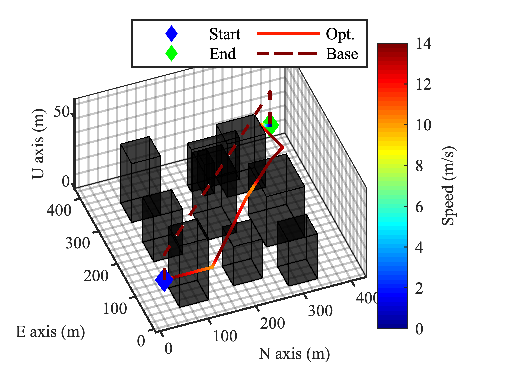
\includegraphics[scale=1.0]{fig13/opt_iso.eps}}
\qquad
\subfloat[The top view of the baseline and optimized path in the drone flight environment.]{\centering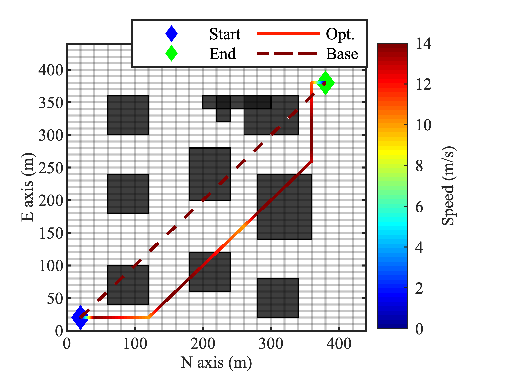
\includegraphics[scale=1.0]{fig13/opt_top.eps}}
\caption{The energy minimum optimization result of drone in the drone flight environment.}
\label{fig: opt_environ}
\end{figure}

The proposed baseline is a path that arrives at the shortest path through linear movement between the starting point and the arrival point using the way point function of drones. The drone in the baseline moves up to the maximum height of the obstacle between the starting point and the end point, then moves straight to the end point and descends to the altitude of the end point. 
In the case of a path derived through optimization, the drone bypasses the obstacles it encounters while flying between the starting point and the end point or moves up to the height of the obstacles to overcome obstacles. 
The movement velocity of drones in the two paths is based on the translational lift effect, which maintains uniform velocity that is minimum energy consumption over distance. 
At baseline, the total power consumption by the drone from the start point to the end point is 49.78 kJ, and the total power consumed by the proposed optimal path is 46.1 kJ, which is 8.4 \% more efficient. The optimal path saves energy by avoiding a sudden increase in motor output, such as bypassing a high level obstacle or overcoming a low level obstacle in a nearby environment instead of overcoming the highest obstacle in the path.
In addition, as the power consumption model used for optimization considers acceleration, the acceleration and deceleration occurring in the drastic direction of drone change considerably change the speed of the drone, which is different from the energy consumption of the existing baseline.
Fig.~\ref{fig:consumed_energy} shows the comparison of consumed energy while going through the generated paths with simulation and with a real experiment. We perform a measurement to verify the fidelity of the simulation result.

\begin{figure}[ht]
\centering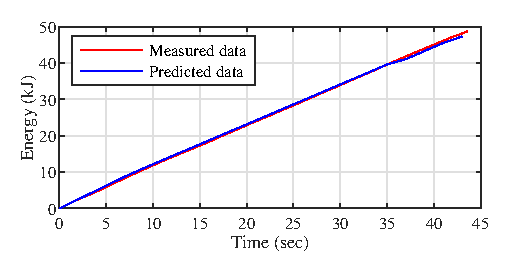
\includegraphics[scale=1.0]{fig14/S_E.eps}
\caption{Comparison of the total energy consumption value by the simulator calculation and M600 flight measurement through travel distance.}
\label{fig:consumed_energy}
\end{figure}

The drone consumes the energy of 48.8 kJ through actual flight experiment and proposed simulation predict the energy consumption of 46.1 kJ.
There is a 5.54~\% difference between the energy consumption predicted by the proposed simulator and the energy consumed by the actual drone.
The validation through the actual flight of the drone shows that the energy consumption of the drone deduced by the proposed simulation and the power consumption of the actual drone are not significantly different.

% 우리는 제시한 최적화 결과를 검증 하기 위하여 시뮬레이션 된 경로를 실제 기체를 통해 주행하였다.
% 실제 실험을 통해 소비한 에너지는 48.8 kJ이며 제안된 방법에 의해서 유추된 에너지는 46.1줄이다. 
% 제안된 시뮬레이터는 실제 드론의 비행과 5.54% 만큼의 에너지 소비에 차이를 보인다. 실제 비행 검증을 통해 시뮬레이션을 통해 드론의 에너지 소모량을 유추하는 것이 실제 드론의 비행과 크게 다르지 않음을 보여준다.



\subsection{Effect of wind on the optimal drone path}

% 앞선 최적화 된 경로는 단순 경로의 변화에서 에너지 소모의 차이를 비교하기 위하여 바람의 영향을 배제 하였지만 비행체를 언급 할 때에는 반드시 바람의 영향이 고려되어야 한다. 바람이 부는 방향에 따라 드론의 비행 경로는 달라져야 하며, 드론의 비행 방향과 바람을 이용하여 에너지 소모를 줄일 수 있을 것이다. 
% 그러나 파워 소비 모델을 형성할 때 와는 다르게 드론에서 실시간으로 바람의 데이터를 제공 받을 방법이 없으므로, 우리는 기상청의 예보처럼 구현 된 환경안에 일정한 바람의 방향과 세기를 설정한다. 이후 바람에 의한 영향을 알기 위해서, 바람에 영향이 존재하는 환경 내에서 드론이 에너지를 최소로 소모하는 경로의 탐색하여, 기존 바람의 영향이 없을 때 탐색 된 최적화 경로와의 에너지 소비량을 비교를 하였다.
% fig 20은 주변 환경의 바람의 세기와 방향에 따라 변화하는 에너지 최적 경로를 각 시점으로 보여준다. 우리는 총 3 가지 케이스에 대하여 적용 되는 바람의 방향의 변화에 따른 최적화 결과를 확인하기 위하여 바람의 방향을 북서쪽, 남동쪽 방향으로 각각 적용하였다. 각 케이스의 베이스 라인은 바람의 영향이 없다고 가정 한 후 도출 한 경로이며, 이 경로에 바람의 방향과 세기를 적용하여 드론이 경로를 따라 비행 하였을 때 소비한 에너지를 계산한다. 그림 내의 모든 최적화 경로는 경로의 변화와 고도의 차이를 확인하기 위하여 사이드 뷰와 탑뷰를 통해 제시 한다.
% fig.20 (a)에서 시작 포인트는 엔드 포인트 보다 고도가 낮으며 생성 된 경로를 통해 드론은 남동 쪽으로 이동한다. 
% 바람의 영향에 의한 경로의 변화를 확인하기 위하여 SE 방향의 바람이 맵 전체에 적용 될 때, baseline과 최적화 경로가 동일하였다. 하지만 두 경로의 에너지 소비는 차이를 보이는데 base line는 41.58 kJ 에너지 소모를 opt는 40.91 kJ의 에너지를 소모하였다. opt 경로는 순 방향의 바람의 영향으로 남쪽으로 진행하는 도중 속도의 변화를 보이며 baseline에 비해 2.25% 에너지를 절약한다.
% 반면 NW 방향의 바람이 적용 될 경우, base line은 62.86 kJ의 에너지를 소모하고 opt는 58.63 kj의 에너지를 소모한다. 바람의 방향이 진행 방향의 역방향 이기 때문에 드론의 에너지 소모가 많이 증가하며 fig.20 (b)와 (c)에서 직관적으로 확인이 가능 할 만큼 경로에 큰 변동이 일어난다. 도출 된 최적 경로는 경로 변화를 통해 baseline 대비 6.73% 의 에너지를 절약한다.

% fig 20.(d) 는 fig.20 (a)와는 다른 경로로 엔드 포인트가 시작 포인트 보다 고도가 높고 드론은 생성 된 경로를 통해 남서 쪽으로 이동한다. 
% 드론의 진행 방향의 측면에 적용되는 바람의 영향으로 모든 최적화 경로에 변화가 생기며, 변화 된 경로에서 드론이 방해물을 넘는 고도와 경로에 따라 에너지 소비의 차이를 보인다.
% 남동 방향의 바람이 적용 될 때 최적화 된 경로와 baseline는 큰 차이를 보이며, baseline은 46.23 kJ, opt는 44.59 kJ의 에너지를 소비하여 opt가 3.55% 효율적이다.
% 대신 북서 방향의 바람이 적용 될 때에는 경로 차이의 폭은 적으나 대각선으로 드론이 상승하는 구간이 길어지는 현상을 보이며 baseline은 50.68 kJ opt는 49.55 kj의 에너지 소모로 opt 가 2.23% 에너지를 절약한다.

% 앞선 2가지 경우와는 다르게 fig.15(g)는 바람이 랜덤하게 배치되었을 때 opt가 어떻게 변하는지를 보여준다.
% 실제 드론이 운용 하는 환경처럼 랜덤한 형태의 바람이 드론의 비행에 영향을 준다고 할 때, 드론의 최적화 경로를 도출 한 것으로 baseline 은 52.29 kJ의 에너지 소비를 opt는 45.65 kJ의 에너지를 소비하여 opt 에서 12.7%의 에너지를 절약한다.

The previous optimized path in Fig.~\ref{fig: opt_environ} excludes the effect of wind to compare the difference in energy consumption in the path changes, but the wind effect must be taken into account when referring to the aircraft.
Depending on the direction of the wind, the flight path of the drone must be different, and the energy consumption of drones can be reduced by using the flight direction of the drone and the wind.
However, unlike when constructing a power consumption model, there is no way to receive wind data in real time, so we set a constant wind direction and speed in an environment constructed like a weather forecast information.
Then, in order to explore the effects of the wind, we search the path that drone consumes the least energy in the environment where the wind effect exist, and compares the energy consumption with the previous optimized path found when there is no existing wind effect.

\begin{figure*}[ht]
\centering
\subfloat[case 1. The wind speed of 6~m/s, the wind direction of NW and SE of, the different altitudes of points, and drone progress of SE direction.]{\centering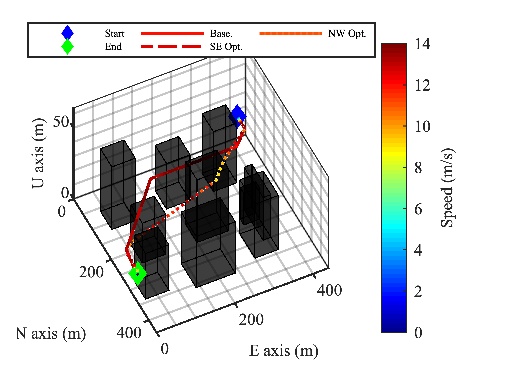
\includegraphics[scale=0.75]{fig15/case1.eps}}
\subfloat[The top view of case 1.]{\centering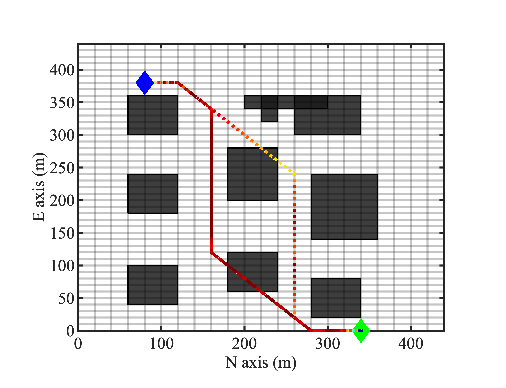
\includegraphics[scale=0.75]{fig15/case1_top.eps}}
\subfloat[The side view of case 1.]{\centering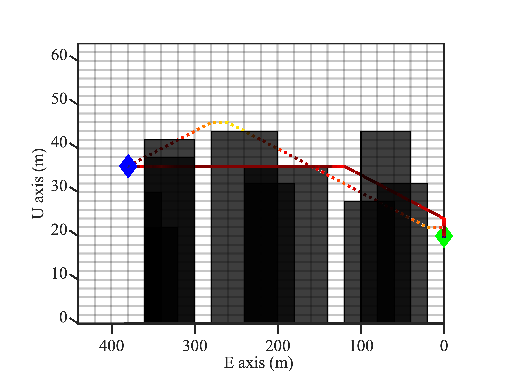
\includegraphics[scale=0.75]{fig15/case1_side.eps}}
\qquad
\subfloat[case 2. The wind speed of 6~m/s, the wind direction of NW and SE of, the different altitudes of points, and drone progress of SW direction.]{\centering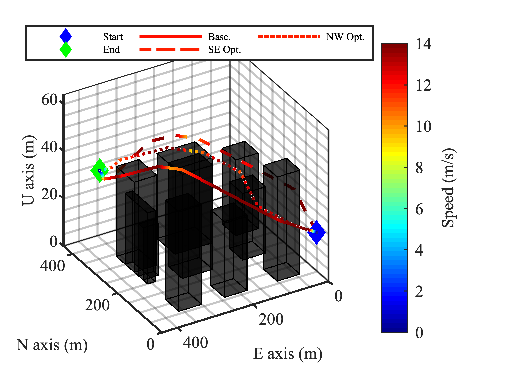
\includegraphics[scale=0.75]{fig15/case2.eps}}
\subfloat[The top view of case 2.]{\centering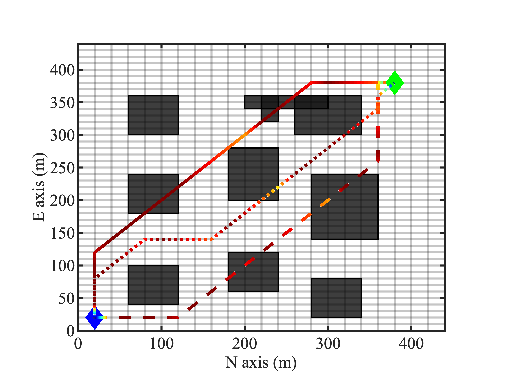
\includegraphics[scale=0.75]{fig15/case2_top.eps}}
\subfloat[The side view of case 2.]{\centering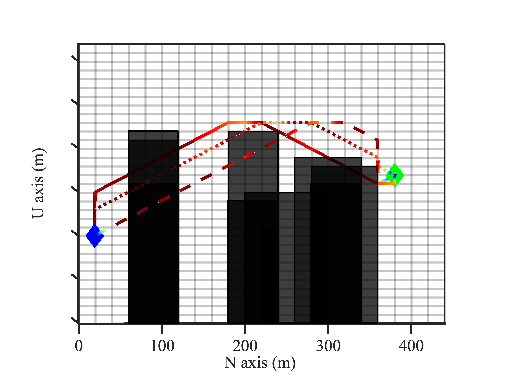
\includegraphics[scale=0.75]{fig15/case2_side.eps}}
\qquad
\subfloat[case 3. The wind speed of 6~m/s, the wind direction of random, the same altitudes of points, and drone progress of SE direction. ]{\centering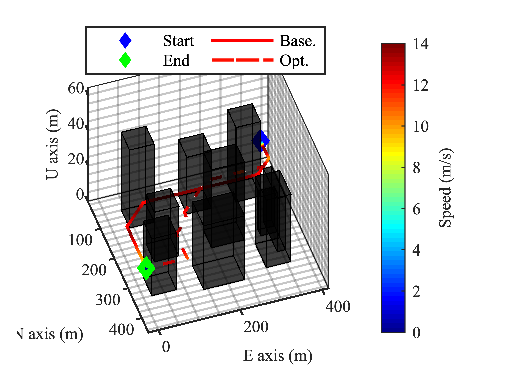
\includegraphics[scale=0.75]{fig15/case3.eps}}
\subfloat[The top view of case 3.]{\centering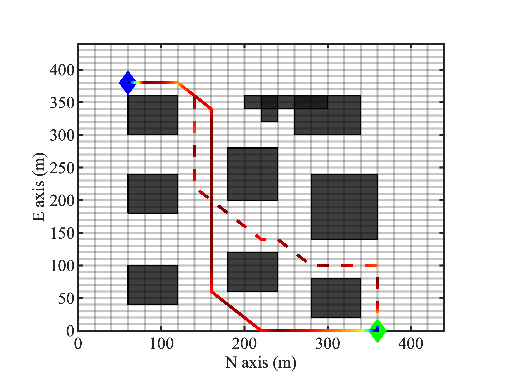
\includegraphics[scale=0.75]{fig15/case3_top.eps}}
\subfloat[The side view of case 3.]{\centering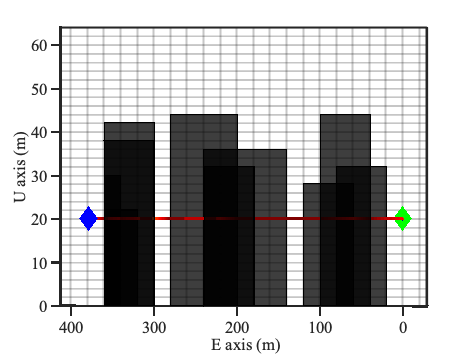
\includegraphics[scale=0.75]{fig15/case3_side.eps}}
\caption{Results of the energy minimum path optimization of drones affected by the wind.}
\label{fig: wind_opt}
\end{figure*}

Fig.~\ref{fig: wind_opt} shows the optimal energy minimum path at each view that changes with the wind speed and direction of the environment. 
We apply the strong wind speed with 6~m/s and the wind direction in the north-west (NW) and south-east (SE) directions, respectively, to confirm the optimization results according to the change in the wind for all three cases. 
The baseline of each case is a path derived after assuming that there is no wind effect as Fig.~\ref{fig: opt_environ}, and calculates the energy consumed when the drone flies along the path by applying wind direction and strength to this path. We present all of optimization paths in the figure as side view and top view to identify the changes in the path and the difference in elevation.

In Fig.~\ref{fig: wind_opt}(a), the start point is lower than the end point and the drone moves south-east direction through the path created. 
First, the baseline and the optimization path are the same when the south-east direction wind are applied to the entire map to confirm the path change due to the wind effect. However, the energy consumption of the two paths differs: the baseline consumes 41.58~kJ and new optimal path considering wind effect consumes 40.91~kJ. 
The optimal path shows a change in velocity with respect to the section compared to the baseline maintaining the speed based on translational lift and saves 2.25~\% energy compared to the baseline.
On the other hand, when wind in the north-west direction is applied, the baseline consumes 62.86~kJ and the optimal path consumes 58.63~kJ.
Since the wind direction is the reverse direction of travel, the energy consumption of the drone increases a lot and the path fluctuates large enough to be intuitively identified in Fig.~\ref{fig: wind_opt}(b) and Fig.~\ref{fig: wind_opt}(c). The derived optimal path saves 6.73~\% of energy compared to the baseline by changing the path.

Fig.~\ref{fig: wind_opt}(d) is a different route than Fig.~\ref{fig: wind_opt}(a), where the endpoint is higher than the starting point and the drone moves southwest through the path created. 
The effect of the wind applied on the side direction of the drone travel causes a change in all optimization paths, with the difference in energy consumption depending on the altitude and path over which the drone crosses the obstacles.  
When the south-east wind is applied, the optimal path and baseline show a big difference of the route, the baseline consumes energy of 46.23~kJ and the optimal path consumes energy of 44.59~kJ, so the optimal path is 3.55~\% efficient then the baseline. 
Instead, when the north-west wind is applied, the path difference is small but the length of the drone rising diagonally is long. the baseline consumes energy of 50.68~kJ and the optimal path consumes energy of 49.55~kJ, so the optimal path saves 2.23~\% of energy then the baseline.

Unlike the previous cases, Fig.~\ref{fig: wind_opt}(g) shows how the optimization path changes when the winds are randomly placed.
Given that random winds affect drones flight, such as the environment in which actual drones operate, the optimal path varies over several intervals. The optimal path consumes the energy of 45.65~kJ and the baseline consumes the energy of 52.29~kJ. The derived optimal path saves 12.7~\% of energy compared to the baseline.










\section{Conclusions}
In this paper, we start from a demonstration that the data provided by the factory on-board power measurement feature of even top-of-the-line commercial drones is highly inaccurate by comparing it with standard equipment. 
This motivates that the power consumption models shown in the previous work may have generated improper predictions compared with the actual power consumption due to the inaccuracy in the measured data.
We implement an accurate in-house on-board power measurement device and collect dozens of hours of power measurement data synchronizing with other flying data. 
Based on the power data, we propose an accurate power consumption model with the deep neural networks (DNNs). 
The proposed power consumption model exhibits error within 10\% compared with a high standard precision data acquisition device. 
The primary benefit of the proposed model is such that i) the model inputs are simple physics parameters of the drone, and external factors affecting power consumption thus it can be easily plugged in various existing optimization framework, and ii) the characterization process is not dependent on the aerodynamics of a particular drone. iii) considering the three-dimensional velocity and acceleration of the drone at the same time, the power consumption of the drone's momentary movement can easily be predicted.
Finally, we demonstrate a example of energy saving by finding an energy efficient path during the operation of a drone using the proposed accurate power consumption model. The optimal path is derived by accurately considering the wind effects that are generally difficult to consider, and the optimal path is 12.7~\% more energy efficient than the general drone operation for random wind effects.











\section{Future works}
% 본 논문은 EDA와 같은 systematic framework로 드론의 단일 기종에 대한 파워 소비 모델과 기본적인 최적화를 진행하였다. 우리가 다음에 할 일은 드론은 다수의 기종을 움직이는 군집 제어가 특징을 활용하기 위해 여러가지 구성이 다른 드론들을 본 논문과 같은 방법으로 파워 모델을 제작하고 최적화를 진행하고자 한다. 각 기종에 대한 드론의 데이터를 쌓은 다음, 쌓여진 데이터를 기반으로 드론의 여러 기종이 움직일 때의 총제적인 운용 비용에 대한 최적화를 진행하고자 한다.

This paper proceeds with the power consumption modeling and energy minimum optimization for a single drone using a systematic framework inspired by EDA technique. Our next work is to create power consumption models and optimize the drones with different configurations in the same way as this paper to apply these optimizations at the cluster control that moves multiple drones. We will accumulate the drone data for different forms of models and then optimize the total operating costs when multiple models of the drone are utilized.










\section*{Acknowledgment}
This work was supported by the National Research Foundation of Korea (NRF-2018R1A2B3007894) and the 2019 Research Fund of Myongji University. 

\bibliographystyle{unsrt}%Used BibTeX style is unsrt
\bibliography{reference}

\begin{IEEEbiography}[{\includegraphics[width=1in,height=1.25in,clip,keepaspectratio]{./bio/dooyoung}}]{Dooyoung Hong}
(S'18) received the B.S. degree in mechanical engineering from Korea University of Technology and Education, Cheonan, Korea in 2017 and received the M.S. degree in the robotics program from Korea Advanced Institute of Science and Technology, Daejeon, Korea in 2019. He is currently pursuing Ph.D. degree in the robotics program, Korea Advanced Institute of Science and Technology. His research interests include low-power embedded system design, and AI based optimization.
\end{IEEEbiography}

\begin{IEEEbiography}[{\includegraphics[width=1in,height=1.25in,clip,keepaspectratio]{./bio/seonhoon}}]{Seonhoon Lee}
(S'18) received the B.S. degree in electrical engineering from Konkuk University, Seoul, Korea in 2018. He is currently pursuing a master’s degree in the school of electrical engineering, Korea Advanced Institute of Science and Technology. His research interests include low-power embedded system, cyber-physical system, and deep learning.
\end{IEEEbiography}

\begin{IEEEbiography}[{\includegraphics[width=1in,height=1.25in,clip,keepaspectratio]{./bio/jaemin}}]{Jaemin Kim}
(S'13 M'18) received the B.S. degree in computer science engineering and the M.S. and Ph.D. degrees in computer science and electrical engineering from Seoul National University, Seoul, Korea, in 2005, 2007, and 2018 respectively. He is currently an assistant professor at the department of electronics engineering, Myongji University. His research interests include low-power embedded system design, electrical energy storage system, and energy soruce reconfiguration system.
\end{IEEEbiography}

\begin{IEEEbiography}[{
%\includegraphics[width=1in,height=1.25in,clip,keepaspectratio]{Bio/nhchang}
}]{Naehyuck Chang}
\end{IEEEbiography}


\end{document}
